\documentclass[journal,12pt,twocolumn]{IEEEtran}

\usepackage{setspace}
\usepackage{gensymb}
\singlespacing
\usepackage[cmex10]{amsmath}

\usepackage{amsthm}

\usepackage{mathrsfs}
\usepackage{txfonts}
\usepackage{stfloats}
\usepackage{bm}
\usepackage{cite}
\usepackage{cases}
\usepackage{subfig}

\usepackage{longtable}
\usepackage{multirow}

\usepackage{enumitem}
\usepackage{mathtools}
\usepackage{steinmetz}
\usepackage{tikz}
\usepackage{circuitikz}
\usepackage{verbatim}
\usepackage{tfrupee}
\usepackage[breaklinks=true]{hyperref}
\usepackage{graphicx}
\usepackage{tkz-euclide}

\usetikzlibrary{calc,math}
\usepackage{listings}
    \usepackage{color}                                            %%
    \usepackage{array}                                            %%
    \usepackage{longtable}                                        %%
    \usepackage{calc}                                             %%
    \usepackage{multirow}                                         %%
    \usepackage{hhline}                                           %%
    \usepackage{ifthen}                                           %%
    \usepackage{lscape}     
\usepackage{multicol}
\usepackage{chngcntr}

\DeclareMathOperator*{\Res}{Res}

\renewcommand\thesection{\arabic{section}}
\renewcommand\thesubsection{\thesection.\arabic{subsection}}
\renewcommand\thesubsubsection{\thesubsection.\arabic{subsubsection}}

\renewcommand\thesectiondis{\arabic{section}}
\renewcommand\thesubsectiondis{\thesectiondis.\arabic{subsection}}
\renewcommand\thesubsubsectiondis{\thesubsectiondis.\arabic{subsubsection}}


\hyphenation{op-tical net-works semi-conduc-tor}
\def\inputGnumericTable{}                                 %%

\lstset{
%language=C,
frame=single, 
breaklines=true,
columns=fullflexible
}
\begin{document}


\newtheorem{theorem}{Theorem}[section]
\newtheorem{problem}{Problem}
\newtheorem{proposition}{Proposition}[section]
\newtheorem{lemma}{Lemma}[section]
\newtheorem{corollary}[theorem]{Corollary}
\newtheorem{example}{Example}[section]
\newtheorem{definition}[problem]{Definition}

\newcommand{\BEQA}{\begin{eqnarray}}
\newcommand{\EEQA}{\end{eqnarray}}
\newcommand{\define}{\stackrel{\triangle}{=}}
\bibliographystyle{IEEEtran}
\raggedbottom
\setlength{\parindent}{0pt}
\providecommand{\mbf}{\mathbf}
\providecommand{\pr}[1]{\ensuremath{\Pr\left(#1\right)}}
\providecommand{\qfunc}[1]{\ensuremath{Q\left(#1\right)}}
\providecommand{\sbrak}[1]{\ensuremath{{}\left[#1\right]}}
\providecommand{\lsbrak}[1]{\ensuremath{{}\left[#1\right.}}
\providecommand{\rsbrak}[1]{\ensuremath{{}\left.#1\right]}}
\providecommand{\brak}[1]{\ensuremath{\left(#1\right)}}
\providecommand{\lbrak}[1]{\ensuremath{\left(#1\right.}}
\providecommand{\rbrak}[1]{\ensuremath{\left.#1\right)}}
\providecommand{\cbrak}[1]{\ensuremath{\left\{#1\right\}}}
\providecommand{\lcbrak}[1]{\ensuremath{\left\{#1\right.}}
\providecommand{\rcbrak}[1]{\ensuremath{\left.#1\right\}}}
\theoremstyle{remark}
\newtheorem{rem}{Remark}
\newcommand{\sgn}{\mathop{\mathrm{sgn}}}
\providecommand{\abs}[1]{\left\vert#1\right\vert}
\providecommand{\res}[1]{\Res\displaylimits_{#1}} 
\providecommand{\norm}[1]{\left\lVert#1\right\rVert}
%\providecommand{\norm}[1]{\lVert#1\rVert}
\providecommand{\mtx}[1]{\mathbf{#1}}
\providecommand{\mean}[1]{E\left[ #1 \right]}
\providecommand{\fourier}{\overset{\mathcal{F}}{ \rightleftharpoons}}
%\providecommand{\hilbert}{\overset{\mathcal{H}}{ \rightleftharpoons}}
\providecommand{\system}{\overset{\mathcal{H}}{ \longleftrightarrow}}
	%\newcommand{\solution}[2]{\textbf{Solution:}{#1}}
\newcommand{\solution}{\noindent \textbf{Solution: }}
\newcommand{\cosec}{\,\text{cosec}\,}
\providecommand{\dec}[2]{\ensuremath{\overset{#1}{\underset{#2}{\gtrless}}}}
\newcommand{\myvec}[1]{\ensuremath{\begin{pmatrix}#1\end{pmatrix}}}
\newcommand{\mydet}[1]{\ensuremath{\begin{vmatrix}#1\end{vmatrix}}}
\numberwithin{equation}{subsection}

\makeatletter
\@addtoreset{figure}{problem}
\makeatother
\let\StandardTheFigure\thefigure
\let\vec\mathbf

\renewcommand{\thefigure}{\theproblem}

\def\putbox#1#2#3{\makebox[0in][l]{\makebox[#1][l]{}\raisebox{\baselineskip}[0in][0in]{\raisebox{#2}[0in][0in]{#3}}}}
     \def\rightbox#1{\makebox[0in][r]{#1}}
     \def\centbox#1{\makebox[0in]{#1}}
     \def\topbox#1{\raisebox{-\baselineskip}[0in][0in]{#1}}
     \def\midbox#1{\raisebox{-0.5\baselineskip}[0in][0in]{#1}}
\vspace{3cm}
\title{Problem}
\author{Sachinkumar Dubey - EE20MTECH11009}
\maketitle
\newpage
\bigskip

\section{Problem}
What conic does the following equation represent.
\begin{align}
y^2-2\sqrt{3}xy+3x^2+6x-4y+5=0
\end{align}
Find the center and equation refered to centre.
\section{Solution}
The general second degree equation can be expressed as follows,
\begin{align}
\Vec{x}^T\Vec{V}\Vec{x}+2\Vec{u}^T\Vec{x}+f=0
\intertext{where,}
\vec{V}=\myvec{3 & -\sqrt{3} \\-\sqrt{3} & 1}\\
\vec{u}=\myvec{3 \\ -2}\\
f=5
\end{align}
Expanding the determinant of $\Vec{V}$ we observe,
\begin{align}
\begin{vmatrix}
2 & -\sqrt{3}\\ 
-\sqrt{3} & 1
\end{vmatrix}=0
\intertext{Also}
\begin{vmatrix}
\vec{V} & \vec{u}\\ 
\vec{u}^T & f
\end{vmatrix}=\begin{vmatrix}
3 &  -\sqrt{3} & 3\\ 
 -\sqrt{3}& 1 & -2\\ 
3 &  -2& 5
\end{vmatrix}\neq0 
\end{align}
Hence we conclude that given equation is a parabola. The characteristic equation of V is given as follows,
\begin{align}
|\vec{V}-\lambda \vec{I}|=0\\
\implies \lambda^2-4\lambda=0 \\
\implies \lambda_1=0,\lambda_2=4
\end{align}
The eigen vector $\vec{p}$ is defined as,
\begin{align}
    (\vec{V}-\lambda \vec{I})\vec{p}=0\\
    \intertext{For \lambda_1=0}
    \myvec{3 & -\sqrt{3} \\-\sqrt{3} &1 }\vec{p}_1=0 \\
    R_2\leftrightarrow \frac{1}{\sqrt{3}}R_1+R_2 \nonumber\\
    \myvec{3 & -\sqrt{3} \\0 & 0}\vec{p}_1=0 \\
    \implies \vec{p}_1=\myvec{1/2 \\ \sqrt{3}/2} \\
    \text{[Choosing Orthonormal eigen vectors]} \nonumber
\end{align}
For $\lambda_2=4$
\begin{align}
    \myvec{-1 -\sqrt{3} \\-\sqrt{3} &-3}\vec{p}_2=0 \\
    R_2\leftrightarrow -\sqrt{3}R_1+R_2 \nonumber\\
    \myvec{3 & -\sqrt{3} \\0 & 0}\vec{p}_2=0 \\
    \implies \vec{p}_2=\myvec{-\sqrt{3}/2 \\ 1/2} \\
    \text{[Choosing Orthonormal eigen vectors]} \nonumber
\end{align}
The matrix $\vec{p}$ is: 
\begin{align}
    \vec{P}=\myvec{ \vec{P}_1& \vec{P}_2}=\myvec{1/2 &-\sqrt{3}/2 \\\sqrt{3}/2& 1/2}\\
    \vec{D}=\myvec{0 &0 \\0& 4}\\
    \eta=2\vec{P}_1^T\vec{u}=2\myvec{3 & -2} \myvec{1/2\\ \sqrt{3}/2} = 3-2\sqrt{3}
\end{align}
The focal length of the parabola is given by:
\begin{align}
\left |\frac{\eta}{\lambda_2}\right |==0.116
\end{align}
When $Det(\vec{V})= 0$, (2.0.1) can be written as
\begin{align}
\vec{y}^T\vec{D}\vec{y}=-\eta \myvec{1 & 0}\vec{y}
\end{align}
And the vertex \vec{c} is given by : 
\begin{align}
\myvec{\vec{u}^T + \frac{\eta}{2} \vec{p}_1^T \\ \vec{V} }\vec{c}=\myvec{ -f\\ \frac{\eta}{2} \vec{p}_1-\vec{u} }
\end{align}
Here,
\begin{align}
\vec{V}=\myvec{3 & -\sqrt{3} \\-\sqrt{3} & 1}\\
\vec{u}=\myvec{3 \\ -2}\\
\vec{p}_1=\myvec{1/2 \\ \sqrt{3}/2}\\
f=5
\end{align}
Putting these value we get:
\begin{align}
\myvec{(3.75-0.5\sqrt{3}) & (-3.5+0.75\sqrt{3})\\3 & -\sqrt{3} \\-\sqrt{3} & 1  }\vec{c}= \nonumber \\ \myvec{ -5\\ \ -2.25-0.5\sqrt{3} \\ 0.5+0.75\sqrt{3}} 
\end{align}
Forming the augmented matrix and row reducing it:
\begin{align}
\myvec{(3.75-0.5\sqrt{3}) & (-3.5+0.75\sqrt{3}) & -5\\3 & -\sqrt{3} & -2.25-0.5\sqrt{3} \\-\sqrt{3} & 1 &0.5+0.75\sqrt{3} }\\
R_3\leftrightarrow -\sqrt{3}R_3 -R_2 \nonumber \\
\myvec{(3.75-0.5\sqrt{3}) & (-3.5+0.75\sqrt{3}) & -5\\3 & -\sqrt{3} & -2.25-0.5\sqrt{3} \\0 & 0 &0}
\end{align}
\begin{align}
    \myvec{2.8840 & -2.2001 & -5\\3 & -1.7320 & -3.1160 \\0 & 0 &0}\\
\myvec{1 & -0.7632 & -1.7337\\3 & -1.7320 & -3.1160 \\0 & 0 &0}\\
\myvec{1 & -0.7632 & -1.7337\\0 & 0.5576 & 2.0851 \\0 & 0 &0}\\
\myvec{1 & -0.7632 & -1.7337\\0 & 1 & 3.7394 \\0 & 0 &0}\\
\myvec{1 & 0 & 1.1202\\0 & 1 & 3.7394 \\0 & 0 &0}
\end{align}
Thus the vertex $\vec{c}$ is:
\begin{align}
\vec{c}=\myvec{ 1.1202\\3.7394} 
\end{align}
\begin{figure}[h!]
    \centering
    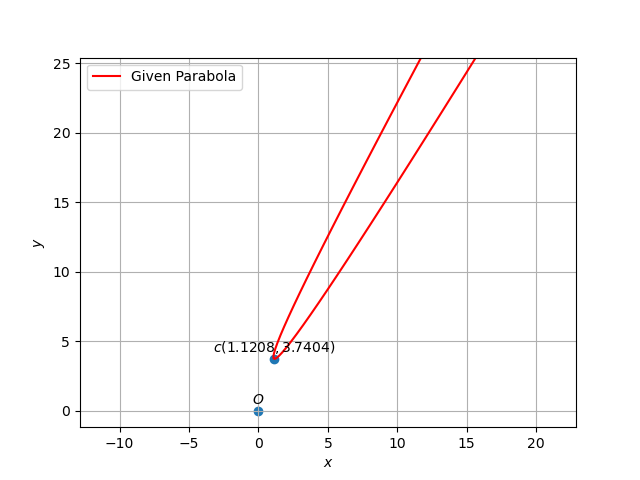
\includegraphics[width=11cm]{Figure_1.png}
    \caption{Plot of the Parabola and its vertex}
    \label{Plot of the Asymtotes}
\end{figure}
\end{document}